\documentclass{article}
\usepackage[utf8]{inputenc}
\usepackage{setspace}
\usepackage{subfig}
\usepackage{graphicx}
\usepackage{tabularx}
\usepackage[T1]{fontenc}
\usepackage{floatrow}
\graphicspath{ {images} }
\doublespacing
\usepackage{pdfpages} 

\usepackage{geometry}
\geometry{
 left=25.4mm,
 top=25.4mm,
 right=25.4mm,
 bottom=25.4mm
 }

\title{Exploration; How Logic Intersects with Uncertainty}
\author{How can classical logic reconcile with epistemic uncertainty?}
\date{April 2022}

\begin{document}

\begin{titlepage}
\maketitle

\begin{center}
Word count: 1901

Stimulus: An image of a computer 

Connection to course: Optional theme of epistemology
\end{center}
\thispagestyle{empty}
\end{titlepage}

\begin{center}
{\huge Stimulus:}


\begin{figure}[h]
    \centering
    \includegraphics[width=8cm]{new1}
    \caption{Stimulus materiel, image of a computer}
    \label{fig:mesh1}
\end{figure}


\end{center}
This is the image of a single board computer. This computer, much like all computers, functions by using a series of logic gates that emulate truth tables with electron configurations inside of its components. In particular it functions off the premise that each logic gate will only receive an 'on' or 'off' state and will process it correctly. These logical computations are done using direct analogs of traditional symbolic logic. For example, the ‘AND’ gate is functionally the same as conjunction statement.

\newpage

I wake up every morning to the shrill tone of my phone alarm, check my messages, and drive to school. Each and every one of those steps including the countless other small intermediate processes rely on the functioning of the computers around me. If they ceased to function for even a second, the order of my day could be turned upside down. Through my investigation of the computer systems that make up this ever-present digital world, one thing became clear. They rely on absolute truth and absolute false to function. In essence, computers are simply logic machines that run on the standard logical system using operators like ‘and’ (conjunction), ‘or’ (disjunction), ‘not’ (negation), and ‘then’ (implication). When these operations fail they fail spectacularly. For example, in 2006 an election was altered in Sweden, when a single computational conjunction operator returned the wrong result (Hammack 2018). These features of computing pose the seemingly obvious question of what if something isn’t true or false.

This may seem like an easy question to answer; everything is either true or false. However, as soon as one looks behind the curtain on why some ideas are considered true it becomes clear that few things, if any, are perfectly true or false because of the nature of knowledge as a far more probable than absolute practise. For example, the statement ‘tomorrow, the sky will be blue’ is very likely true, but because it hasn’t happened yet, it possesses some kind of chronological uncertainty in the same way that all things that haven’t happened yet do. 

Most philosophers and logicians have settled into one of two camps. The first is those who believe in bivalence. This set of philosophers will generally tell you that all logical statements can be categorized as true or false, with no middle values (Dennett, 2016). Specifically, those who only believe in 2-valued logics are termed monists. The second are those who believe in many-valued logic. They will tell you that there is at least one value that isn’t true or false. Though this is where the real discussion happens because of the multitude of answers to that guiding question. In fact, there are so many that they are simply categorized as ‘non-standard’ logic. 

What becomes clear is that there is a strong need to quantify this ‘non-standard’ logic into something that can be worked with by computers and humans alike. So far, two things are established: uncertainty exists, and that uncertainty needs to be factored into any logical perspective of the world (like that of computers). Currently, this is done through one primary method, simply evaluating against a threshold to determine the truth of a statement (otherwise called “threshold logic”). Rather than attempt to propagate uncertainty through each statement, evaluate each premise or variable of the statement at some threshold to collapse it into a bivalent (true or false) state where traditional logic can function (Wyatt 2021). This approach is, however, fundamentally flawed because it chooses to ignore almost all of the complexity present in our world by using some arbitrary threshold for true or false. Say that a scientist knows that there is an 80\% chance that some arbitrary event has passed. Would it be reasonable to ask if that event had happened and only accept true or false as answers? Of course not, this is ridiculous precisely because it removes the degree of uncertainty that is key to the truth. By only accepting true and false, the statement attempts to remove the probabilistic nature of the world by abstracting it away with true and false. All things in our universe obey simple probabilistic principles, so ignoring those probabilities necessarily impedes the creation of cogent logic or tautologies.

There are a few attempts to reconcile traditional logic with uncertainty. The first was done by Jan Łukasiewicz in the 1920s through his unpublished work (Gottwald 2015). His approach has since been termed modal logic since it adds an intermediate value. He proposed a third value, one of uncertainty. Where not only is there true and false, but also some third value to represent uncertainty of all types. There are a few flaws in this line of reasoning because it assumes that all types and quantities of uncertainty are the same. That is to say, the statement ‘this document contains no German spelling errors’ and ‘we exist in a multiverse’ are treated exactly the same despite one being almost certainly true and the other being almost unknowable . The second main flaw is that no matter how you quantify uncertainty, the different types of uncertainty result in fundamentally different truth tables. For example, both of the tables below are emergent dependent on your interpretation of uncertainty.


\begin{figure}[!ht]
    \centering
    \begin{floatrow}
      \ffigbox[\FBwidth]{\caption{Kleen's interpretation}\label{fig:kleen}}{%
        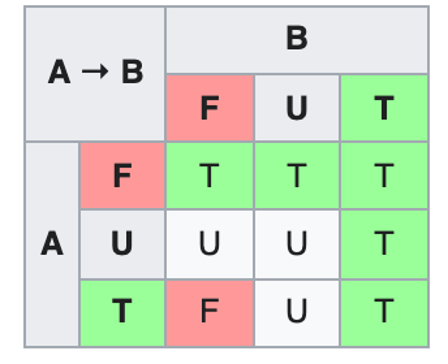
\includegraphics[width=7cm]{/left.png}   % Just a dummy. Replace with your figure.
      }
      \ffigbox[\FBwidth]{\caption{Łukasiewicz's interpretation}\label{fig:luka}}{%
        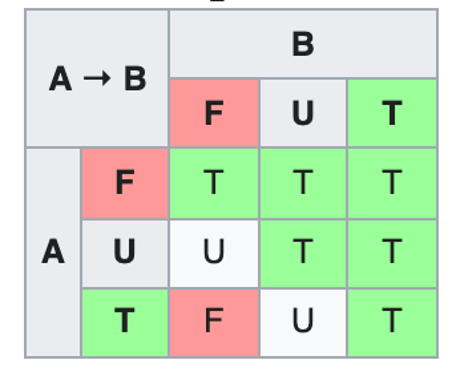
\includegraphics[width=7cm]{/right.png}   % Just a dummy. Replace with your figure.
      }
    \end{floatrow}
\end{figure}


Both interpretations are nearly identical, except for the statement $U\Rightarrow U$. Figure \ref{fig:kleen} is a far more traditional understanding than if you are talking about uncertainties then the result will necessarily be uncertain. An example of this interpretation might be ‘if a train leaves the station tomorrow, then the moon will be green tomorrow’. Obviously, because both variables are uncertain, the result will be uncertain. However, figure \ref{fig:luka} seems to indicate that this could be a true statement. For example, ‘if the train leaves the station tomorrow, then the train will have left the station tomorrow morning’. This statement seems to point towards the second interpretation of uncertainty. This is only the beginning considering that both of these logics have strong and weak variants for the combinations of true, false, and uncertain. For each of these interpretations, a set of logical statements can exist to support them much like these two. In this case, because there are multiple systems that break down in certain cases, but prove correct in certain circumstances, it points towards some underlying truth table that differentiates between each of these cases.

This led to something of a new idea, what if the properties of truth and falsity exist on a continuous spectrum, rather than simply complying with the limited values provided by 2 and 3 values logics. This is where the work of two philosophers/mathematicians/logicians becomes key. Throughout the 20th century, Gödel and Łukasiewicz led the field on many-valued logics. Both of their logics center around how one could interpret truth values between zero and one. They differentiate in a few key ways. Firstly, Gödel treats negation as an operation to collapse any premises into a true or a false case, whereas Łukasiewicz uses the negation operator to reflect the truth value across the midpoint of true and false (Aloni, 2016). The table below illustrates this difference using a premise that is 0.60 true. 

\begin{center}
\begin{tabularx}{0.8\textwidth} { 
  | >{\centering\arraybackslash}X 
  | >{\centering\arraybackslash}X  | }
 \hline
 Gödel ($G_\infty$) &  Łukasiewicz ($L_\infty$) \\
 \hline
 ¬0.6 = 0  & ¬0.6 = 0.4  \\
\hline
\end{tabularx}
\end{center}

This is indicative of the type of thinking that leads to both of these logics. Gödel attempts to collapse the state of each premise as much as possible. His approach is to limit the impact that uncertainty can have on any statement to result in an absolutely true or false result most of the time. Łukasiewicz, starkly opposing Gödel, uses the principles of symmetry to come to his conclusions. This is evident in the negation operator where he simply swaps the property of true and false, though it is prevalent in all operators of his logic. Łukasiewicz’s logic is highly assumptive that true and false are perfect opposites. This can be called into doubt because his logic doesn’t explicitly state what exactly this range from 0 to 1 means or why a step from 0.1 to 0.2 is fungible with a step from 0.8 to 0.9. Without explicitly stating how this truth value is derived, it is unclear that they prosses and symmetrical properties. 

That’s not to say that Gödel’s system is more correct though. Much like Łukasiewicz he also deals mainly in the conceptuality of uncertainty rather than the actual derivation of those values. His logic specifically doesn’t match one key property that double negation should have the same identity as any original statement. This means that ¬¬P is not always equivalent to P (Zach R et al 2020). This breaks most if not all applications of this type of logic because this means that applying operators in some equivalent way won’t provide an equivalent result.

Much like in the case of 3 valued logic, the fact that they both have cases in which they are correct and cases in which they return the wrong result alludes to some underlying more fundamental issue that can’t just be resolved by increasing the number of degrees of truth. So far this has stumped some of the brightest minds in logic and has led to a variety of other non-classical variations of Aristotle’s original logic like quantum logic, non-reflexive logic, and paraconsistent logic. Each of these systems attempts to address one or more fundamental flaws in tradition, modal, and many-valued logics.

Since all of these logics seem to share one fundamental issue with the way that they consider all types of uncertainty fungible. It is clear to me that any solution must differentiate between different types of uncertainty. For example, epistemic, definitional, and chronological uncertainty should all be treated separately. It is clear to me that the solution is to create a system where we differentiate between true, and false, as well as each type of uncertainty. To put this into logical terms, each premise should be a combination of separate uncertainties. For example, the statement ‘the sky will be blue tomorrow’ should have chronological uncertainty because it hasn’t happened yet, definitionally uncertainty because blue is purely subjective, and every type of uncertainty that could impact it. However, identifying every type of uncertainty and quantifying them is a highly intractable problem. Ideally, we would apply the rules presented in Łukasiewicz’s logic in a property-wise fashion so that any conclusions include all of the types of uncertainty already presented.

No matter how much you break uncertainty down into its parts, the issue of symmetry remains unaddressed. For this reason, I think it is far more accurate to characterize true and false separately. This means that you could use a spectrum of -1 to 1 instead of 0 to 1. This could be any experiment where it is far easier to prove truth than falsity or vice versa. For example, the statement, ‘there is a toaster in orbit around the sun' is far easier proved than disproved because proving it is as simple as a photo, whereas a disproof would involve a comprehensive survey of all of space. This in combination with connecting the value to the possibility rather than some arbitrary value could be far more useful. So instead of setting an arbitrary value of 0.1 to ‘a ship will sail tomorrow’, we would attempt to evaluate the possibility of such a thing happening.

Though this is far from my own logical calculus, it’s clear now that the approach taken by philosophers like Gödel and Łukasiewicz, while very useful, are limited by their unclear definitions of uncertainty and their treatment of uncertainty as one cohesive similar issue. Any solution to the problem of formalizing uncertain non-classical logic must either consider these in a similar way to myself through a probabilistic lens or reimagine logic entirely (possibly from a deterministic standpoint). The only thing I am certain of now, is that I should be certain of nothing.


\includepdf[pages=2]{ref.pdf}

\end{document}
